% !TEX root = ../../main.tex


\begin{figure}[tb]
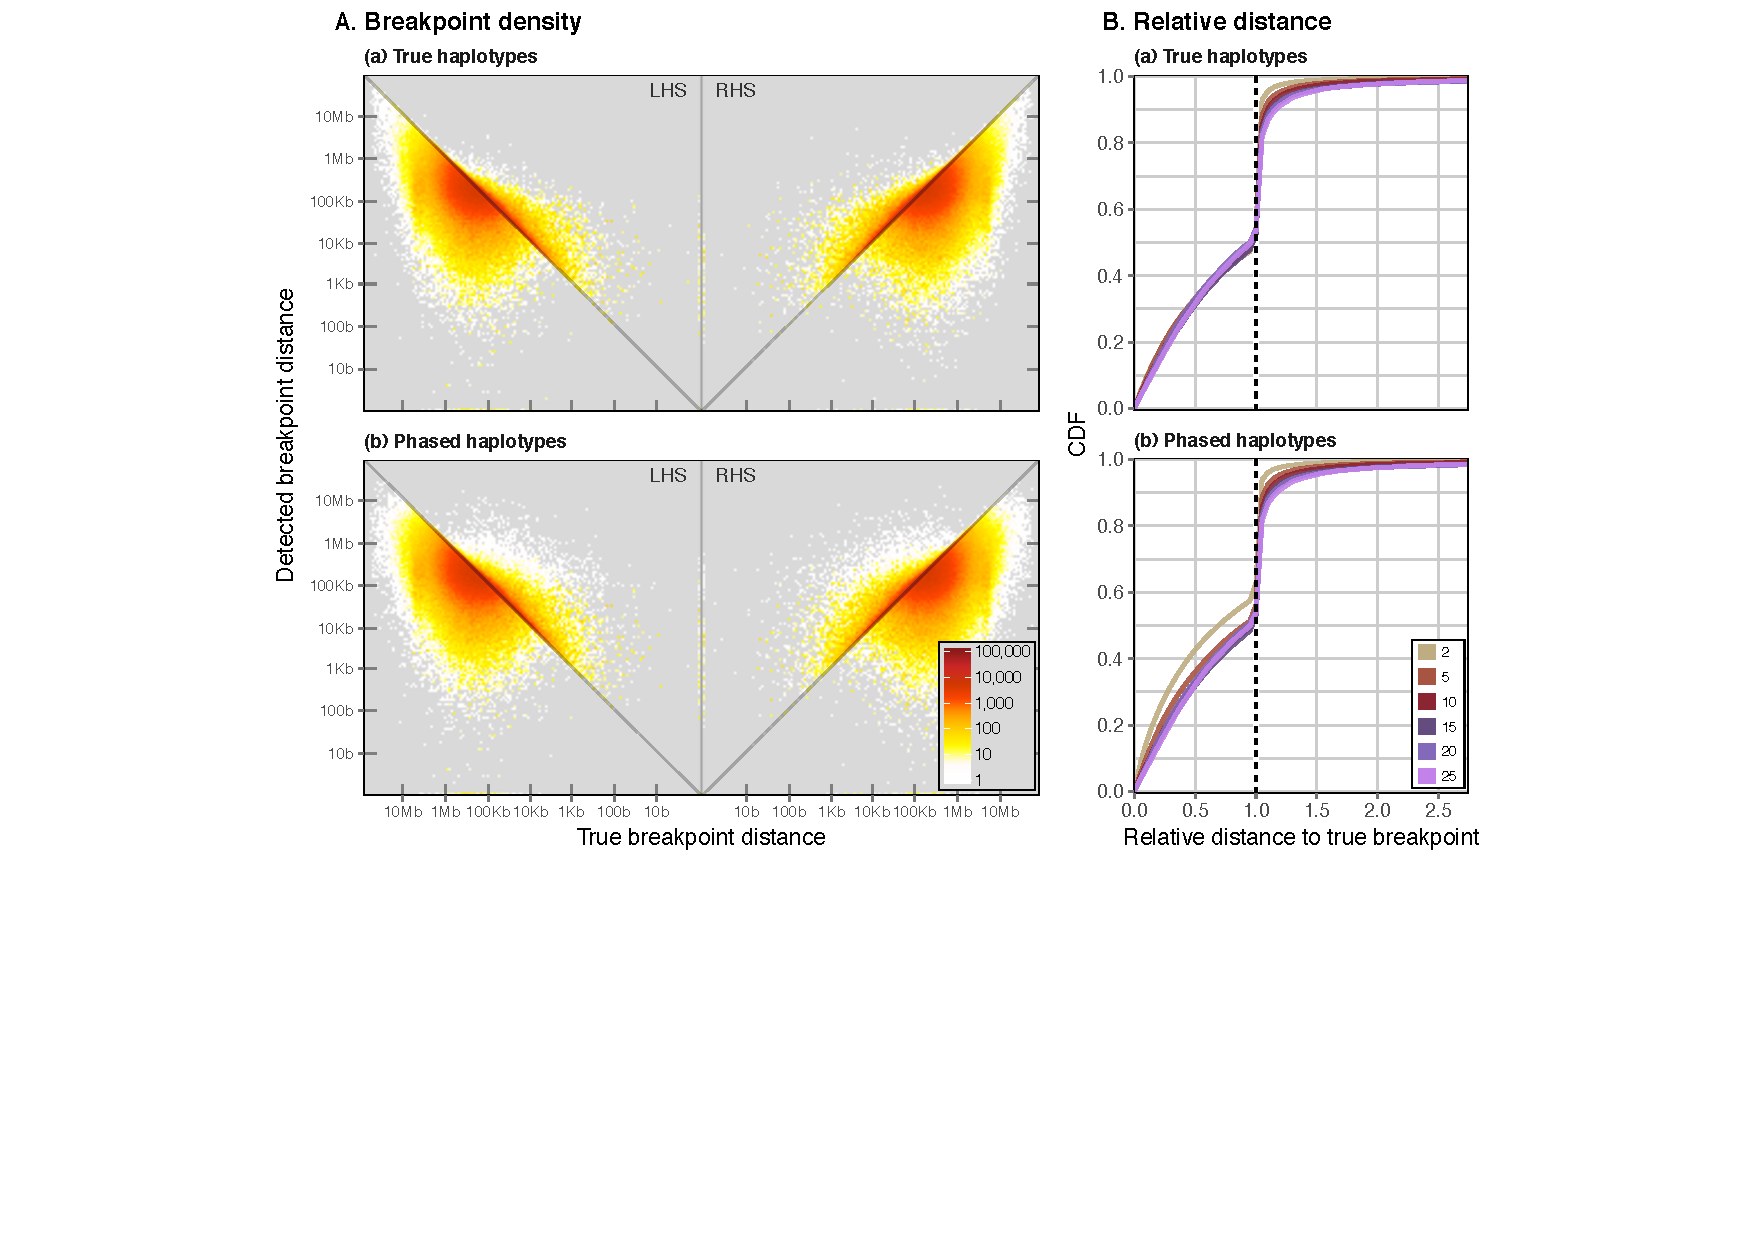
\includegraphics[width=\textwidth]{./img/ch3/beagle_break_tru_new}
\Caption{Accuracy of breakpoint detection using \emph{Refined\,IBD} in Beagle~4.1}
{Results are shown for shared haplotype segments inferred using the \texttt{Refined\,IBD} method; after the detected segments were matched to the set of true segments based on a given target site being contained within the interval of the detected segment.
IBD was inferred on true (simulated) haplotype data \textbf{(a)} and phased haplotypes \textbf{(b)}.
Panel~\textbf{(A)} provides a heatmap representation of a scatter plot, comparing physical distances between focal site and true breakpoint (x-axis) and detected breakpoint (y-axis).
Segment breakpoints to the left (\emph{LHS}) and right-and side (\emph{RHS}) of the focal position are shown separately.
Panel~\textbf{(B)} shows the \gls{cdf} of detected breakpoints in relative distance to the focal and true breakpoint sites.\CorrectLabel}
{fig:beagle_break_tru}
% \vspace{-5pt}
% \hrulefill%
\end{figure}
